\documentclass[11pt]{article}
\usepackage[a4paper,margin=0.85in]{geometry}
\usepackage{amsmath,amssymb,booktabs,graphicx,tabularx,longtable,microtype}
\usepackage[hidelinks]{hyperref}
\title{Work Package 9: Unified Monte Carlo and Computational Validation\\\large Reproducibility appendix for causal operator interventions in linear SPDEs}
\author{}
\date{7 July 2026}
\begin{document}
\maketitle
\begin{abstract}
This appendix validates the complete WP3--WP8 theorem chain using an exact spectral simulation of the stochastic heat equation, deterministic Gaussian law calculations, and constructive non-identification experiments. The original Cartesian $(N,n)$ design is audited against the heat-equation resolution condition and replaced, for inferential validation, by a theorem-aligned paired design with 1,000 replications per cell. The suite reports estimator bias and RMSE, mixed-rate LAN diagnostics, counterfactual CDF and quantile errors, pointwise and simultaneous coverage, multiplier sensitivity, Galerkin and temporal slopes, total-error balancing, operator derivatives, and factual-merging/counterfactual-separation failures. A clean one-command execution completed in 67.1 seconds and records raw data, software versions, Git provenance, and SHA-256 checksums.
\end{abstract}

\section{Design audit}
For the Dirichlet heat equation on $(0,1)$,
\[
 \lambda_N\Delta_n=\pi^2N^2/n.
\]
Only 1 of 25 planned Cartesian cells satisfy the operational threshold $\lambda_N\Delta_n\le0.15$. The high-replication designs are $(5,2000)$, $(10,8000)$, and $(20,32000)$, each with 1,000 replications and $\lambda_N\Delta_n=0.123370$.

\section{Estimation and LAN}
\resizebox{\textwidth}{!}{%
\begin{tabular}{llllllllllllll}
\toprule
N & n & lambda\_N\_Delta & theta\_bias & theta\_rmse & theta\_empirical\_sd & theta\_average\_se & sigma\_bias & sigma\_rmse & sigma\_empirical\_sd & sigma\_average\_se & ztheta\_sd & zsigma\_sd & scaled\_cross\_correlation \\
\midrule
5 & 2000 & 0.1234 & 0.003414 & 0.02416 & 0.02393 & 0.0237 & 6.581e-05 & 0.002134 & 0.002134 & 0.002122 & 1.018 & 1.006 & 0.07463 \\
10 & 8000 & 0.1234 & 0.0004481 & 0.009086 & 0.00908 & 0.008895 & 2.415e-05 & 0.0007493 & 0.0007493 & 0.0007501 & 1.022 & 0.999 & 0.0966 \\
20 & 3.2e+04 & 0.1234 & -9.863e-05 & 0.003253 & 0.003253 & 0.003253 & 6.925e-06 & 0.0002639 & 0.000264 & 0.0002652 & 0.9995 & 0.9955 & 0.1222 \\
\bottomrule
\end{tabular}
}%

The information-standardised empirical standard deviations differ from one by at most 0.0219. Figures~\ref{fig:hist}--\ref{fig:lr} display the normal and likelihood-ratio diagnostics.

\begin{figure}[ht]
\centering
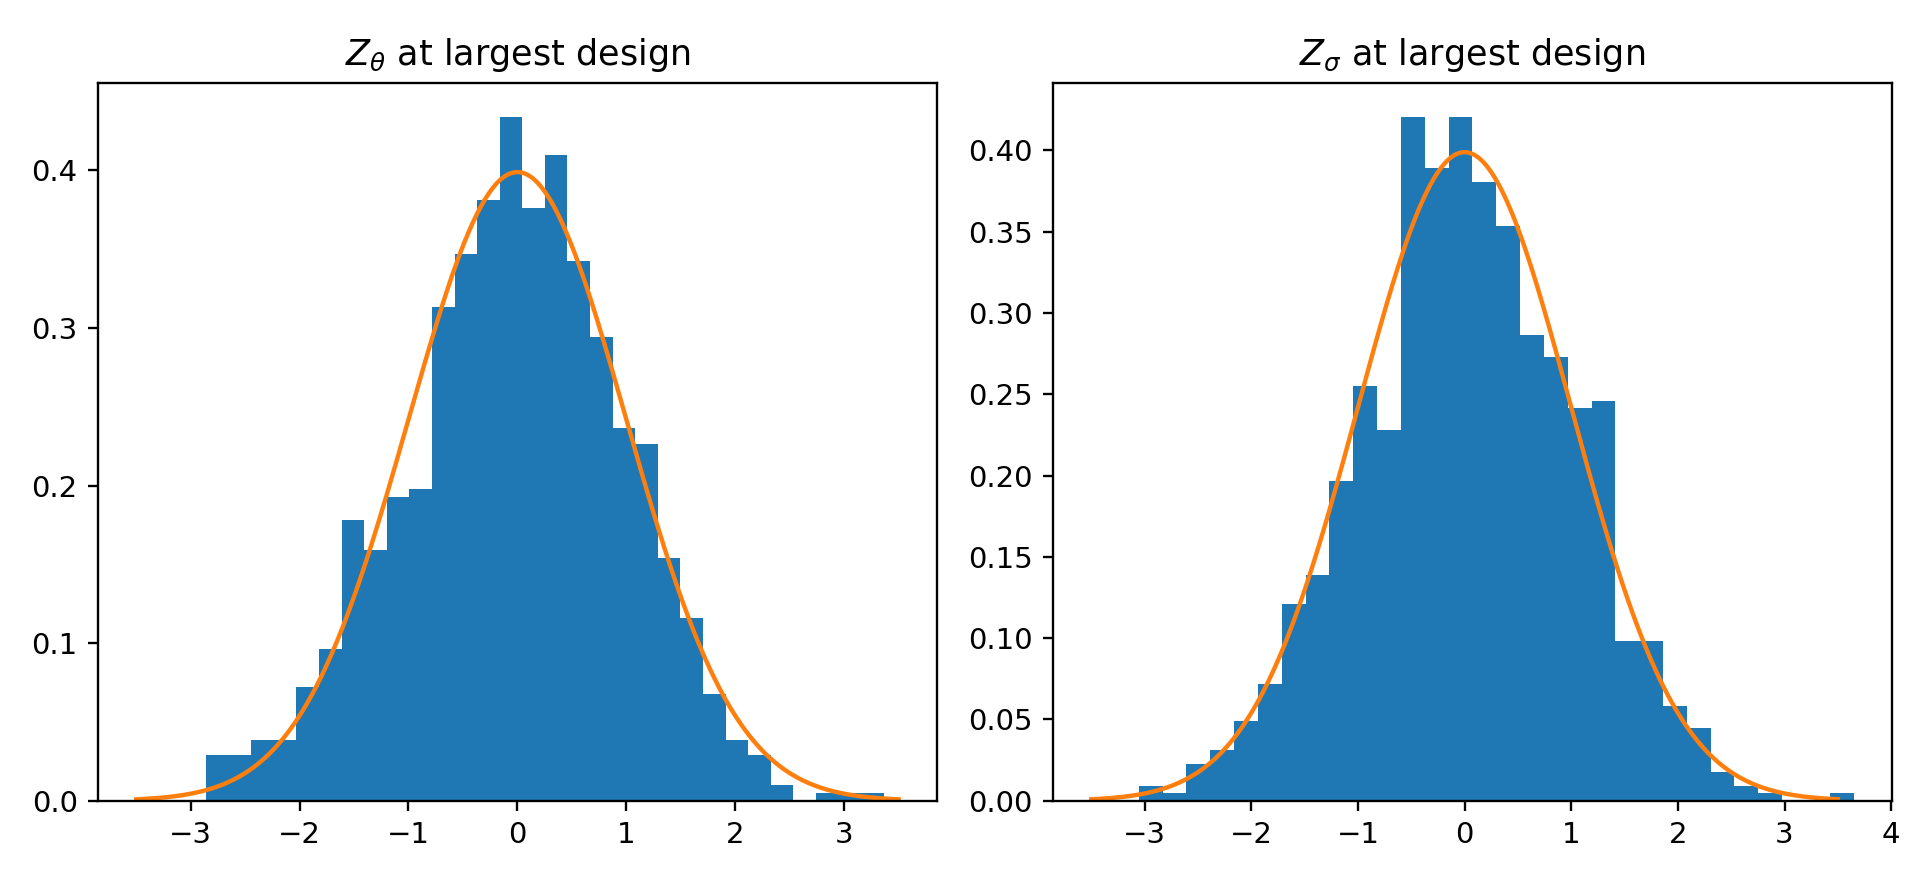
\includegraphics[width=.82\textwidth]{../results/figures/lan_histograms.png}
\caption{Information-standardised estimator histograms at the largest theorem-aligned design.}
\label{fig:hist}
\end{figure}

\begin{figure}[ht]
\centering
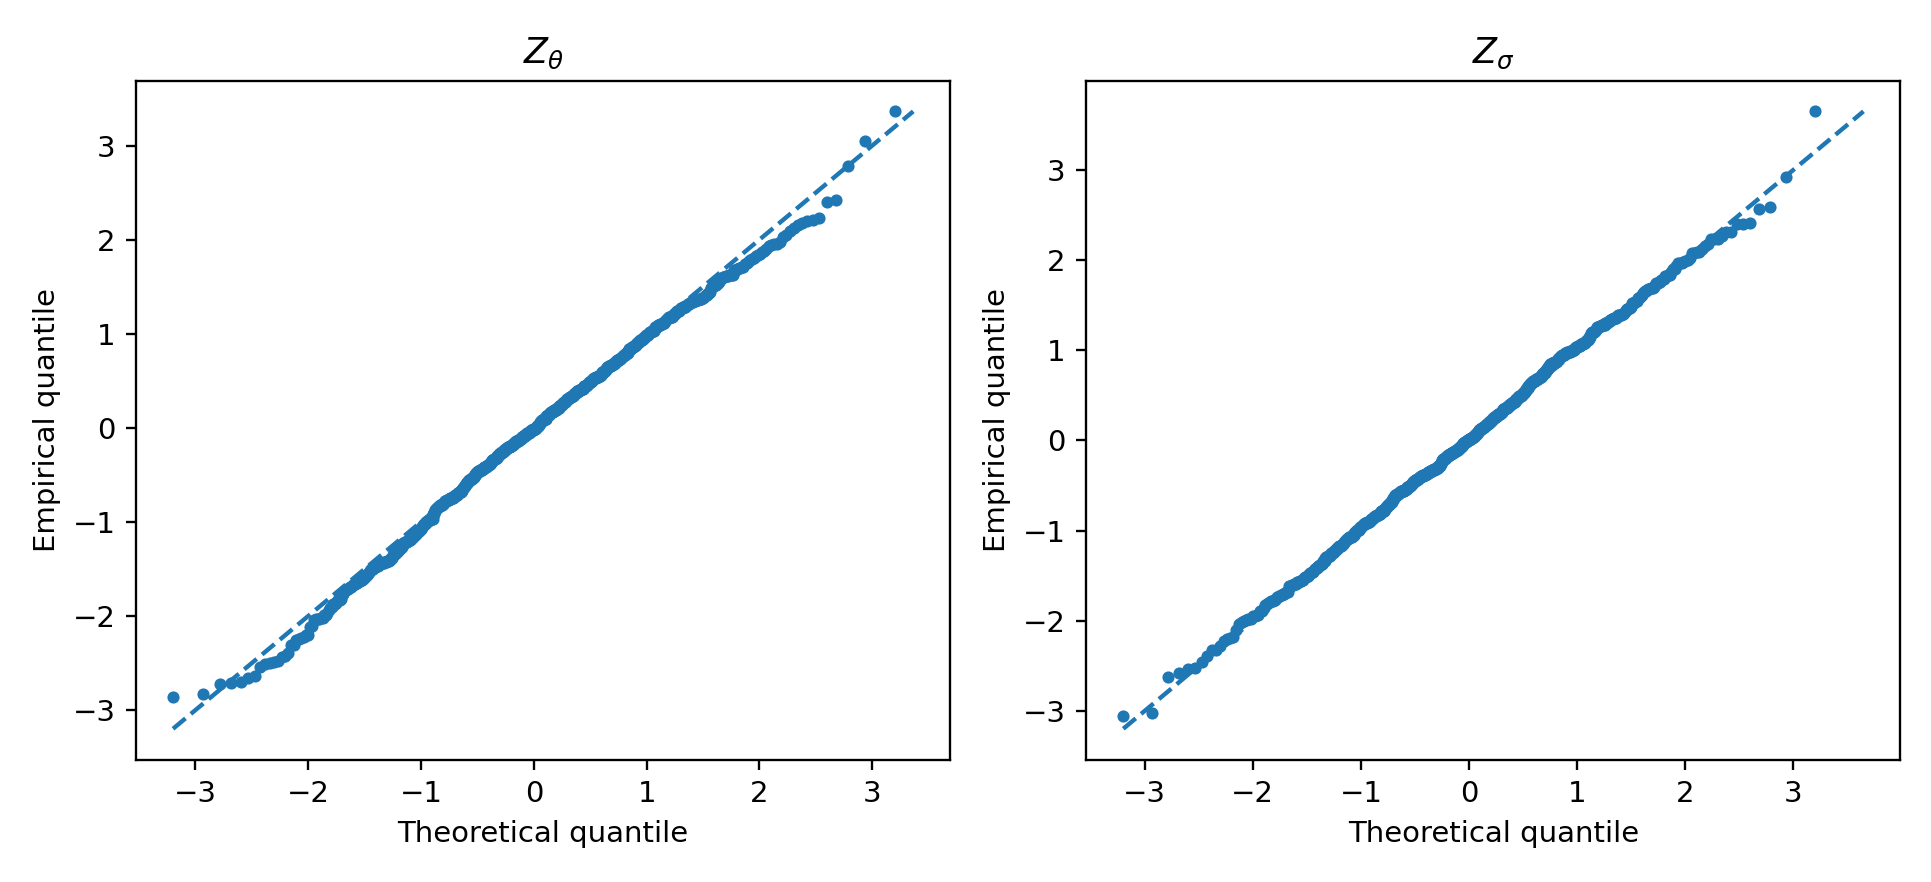
\includegraphics[width=.82\textwidth]{../results/figures/lan_qq_plots.png}
\caption{Normal quantile diagnostics for the mixed-rate estimators.}
\end{figure}

\begin{figure}[ht]
\centering
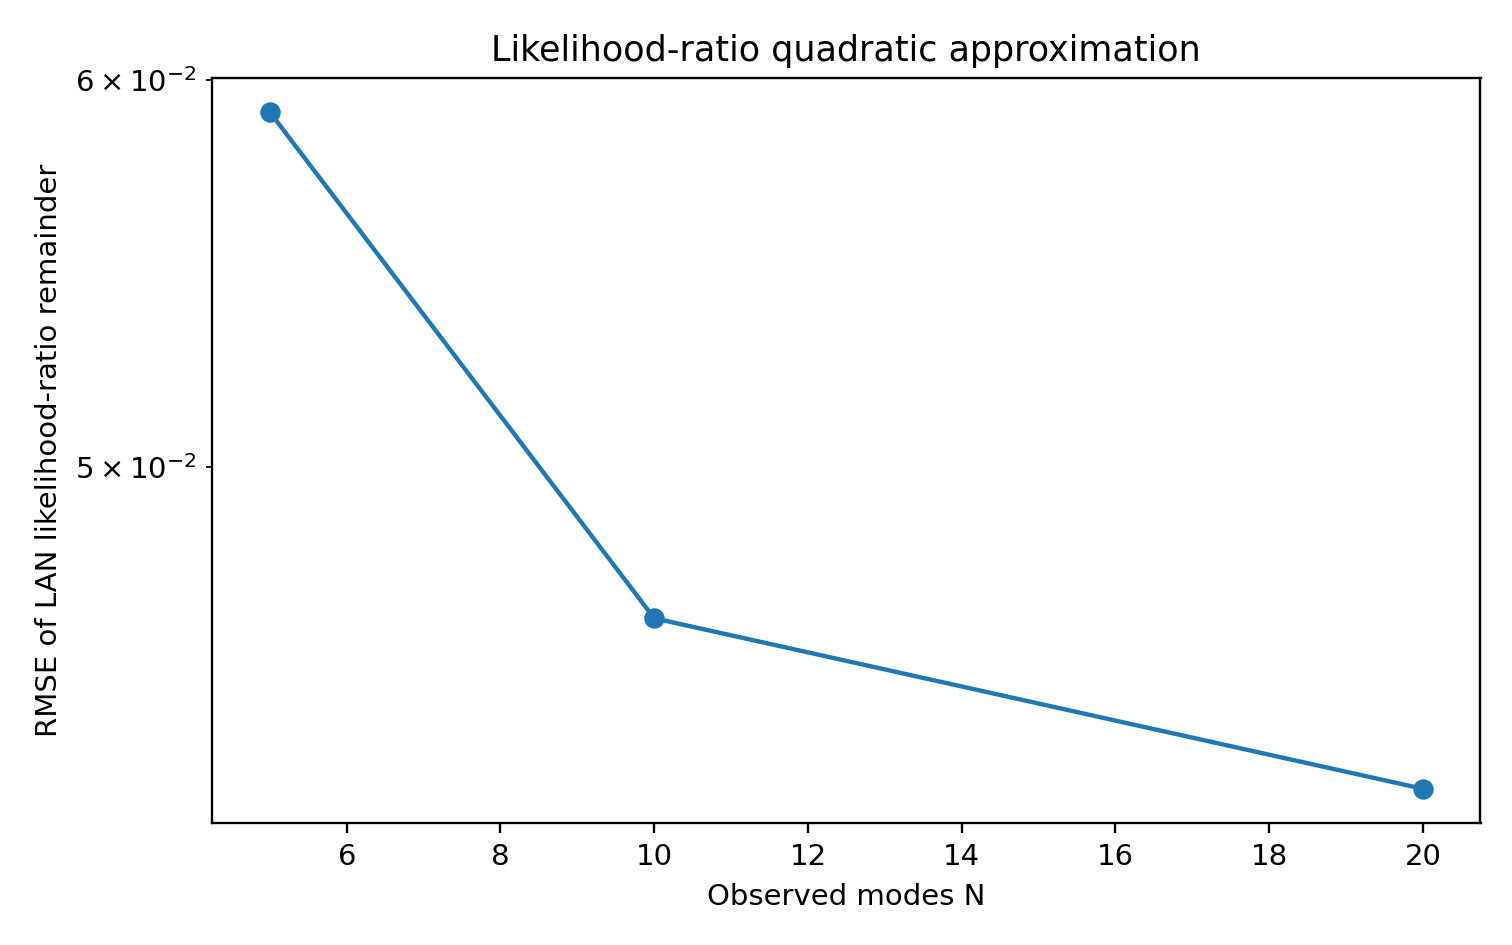
\includegraphics[width=.72\textwidth]{../results/figures/lan_likelihood_ratio_remainder.png}
\caption{RMSE of the LAN likelihood-ratio quadratic remainder.}
\label{fig:lr}
\end{figure}

\section{Counterfactual targets and bands}
\resizebox{\textwidth}{!}{%
\begin{tabular}{llllllllll}
\toprule
N & n & cdf\_sup\_rmse & effect\_sup\_rmse & fast\_simultaneous\_coverage & slow\_simultaneous\_coverage & fast\_average\_full\_width & slow\_average\_full\_width & pointwise\_coverage\_min & pointwise\_coverage\_max \\
\midrule
5 & 2000 & 0.00172 & 0.01639 & 0.946 & 0.95 & 0.006707 & 0.06374 & 0.945 & 1 \\
10 & 8000 & 0.0006043 & 0.006286 & 0.955 & 0.948 & 0.002371 & 0.02417 & 0.955 & 1 \\
20 & 3.2e+04 & 0.0002129 & 0.002261 & 0.951 & 0.951 & 0.0008384 & 0.008856 & 0.951 & 1 \\
\bottomrule
\end{tabular}
}%


\begin{figure}[ht]
\centering
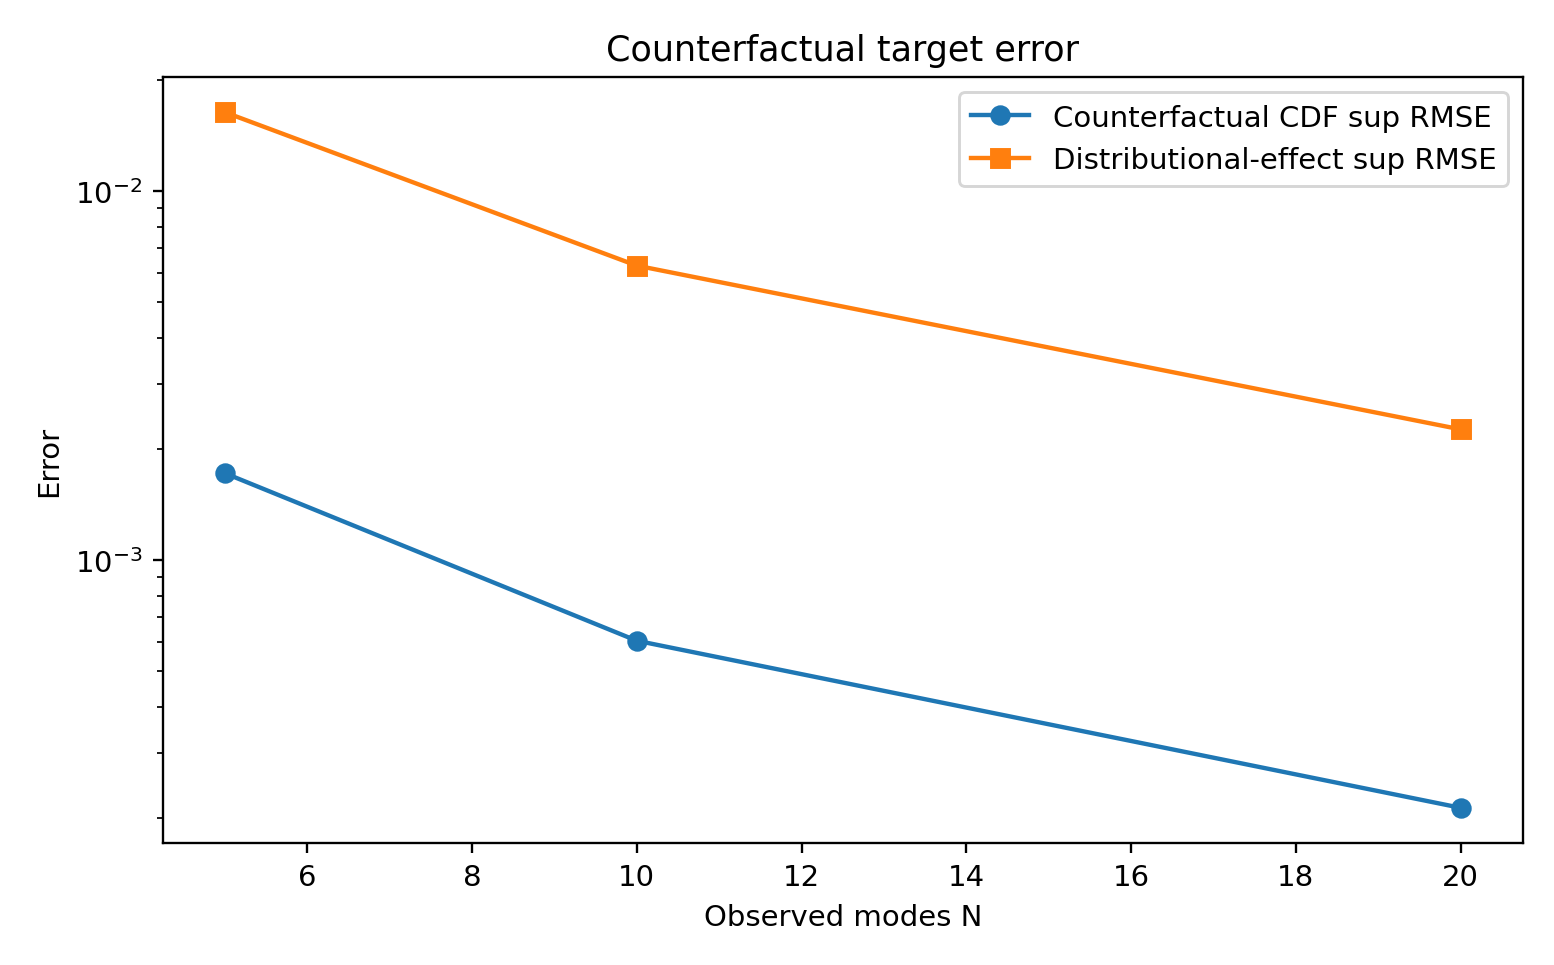
\includegraphics[width=.74\textwidth]{../results/figures/counterfactual_target_errors.png}
\caption{Contraction of fixed-intervention CDF and factual-versus-counterfactual effect errors.}
\end{figure}

\begin{figure}[ht]
\centering
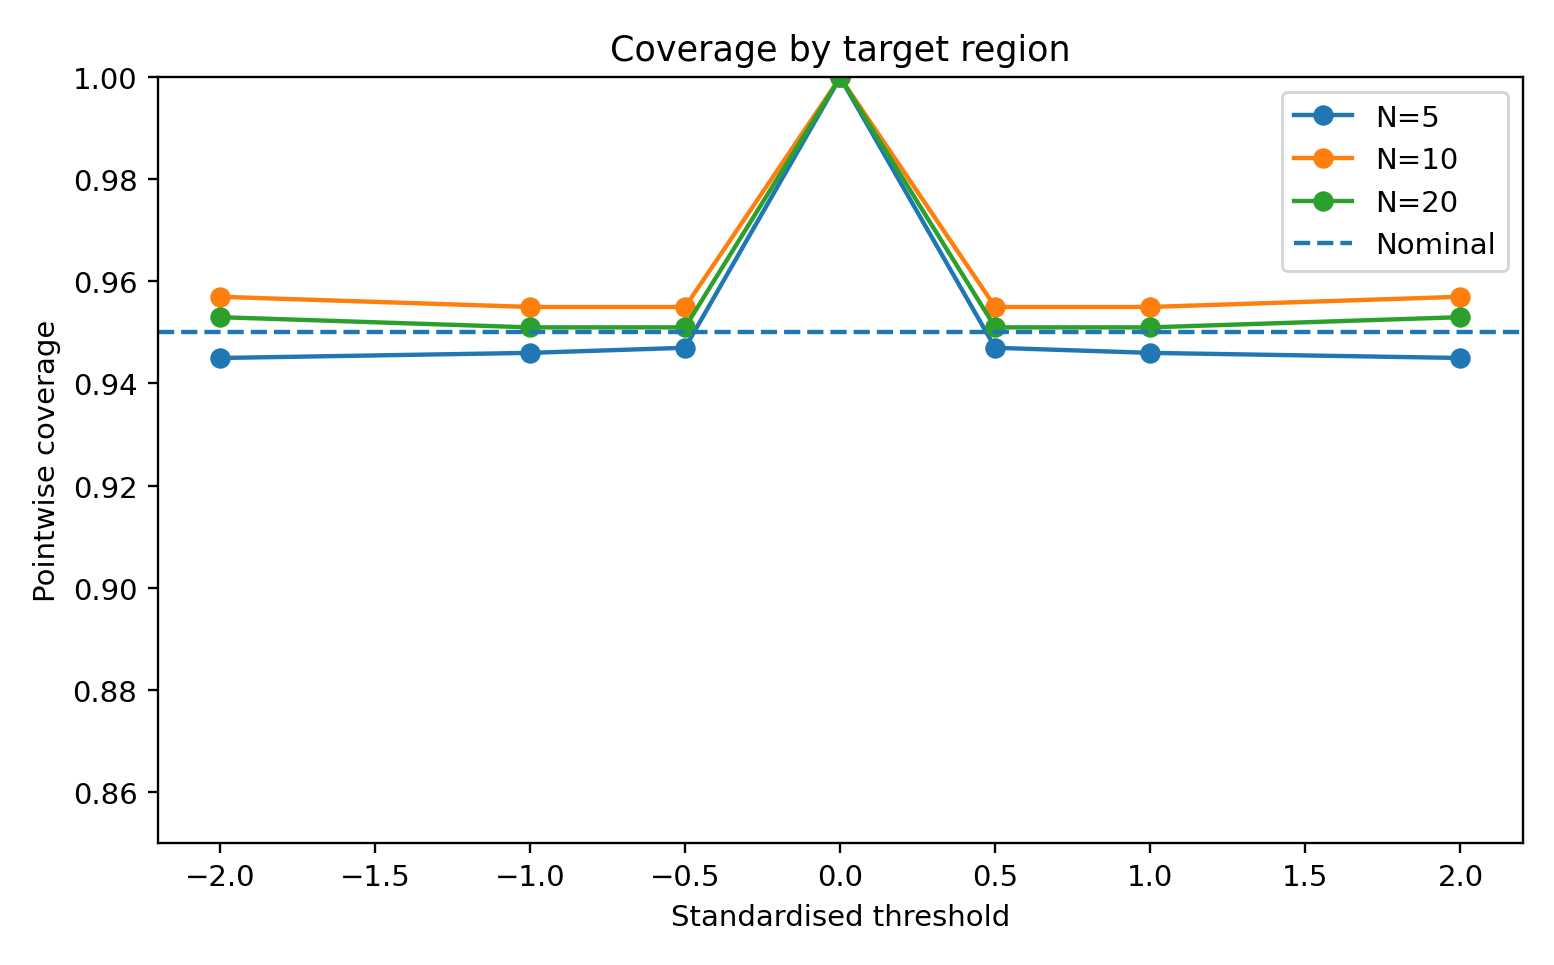
\includegraphics[width=.74\textwidth]{../results/figures/pointwise_coverage_by_threshold.png}
\caption{Pointwise coverage over central and tail threshold regions.}
\end{figure}

\section{Bootstrap sensitivity}
\resizebox{\textwidth}{!}{%
\begin{tabular}{llllllll}
\toprule
sensitivity\_axis & method & draws & grid\_size & fast\_coverage & slow\_coverage & fast\_mean\_full\_width & slow\_mean\_full\_width \\
\midrule
multiplier & direct\_gaussian & 499 & 31 & 0.9333 & 0.93 & 0.002351 & 0.02412 \\
multiplier & mode\_gaussian & 499 & 31 & 0.96 & 0.9467 & 0.003021 & 0.03424 \\
multiplier & mode\_rademacher & 499 & 31 & 0.9567 & 0.9467 & 0.002943 & 0.03279 \\
draw\_count & direct\_gaussian & 199 & 31 & 0.94 & 0.9367 & 0.00235 & 0.02385 \\
draw\_count & direct\_gaussian & 999 & 31 & 0.94 & 0.9267 & 0.002375 & 0.02415 \\
grid\_resolution & direct\_gaussian & 499 & 11 & 0.9333 & 0.9267 & 0.002361 & 0.02407 \\
grid\_resolution & direct\_gaussian & 499 & 61 & 0.9367 & 0.92 & 0.002369 & 0.0241 \\
\bottomrule
\end{tabular}
}%

The mode-block procedures are mildly conservative at finite $N$, while the direct Gaussian multiplier is narrower because the limiting covariance is known analytically.

\begin{figure}[ht]
\centering
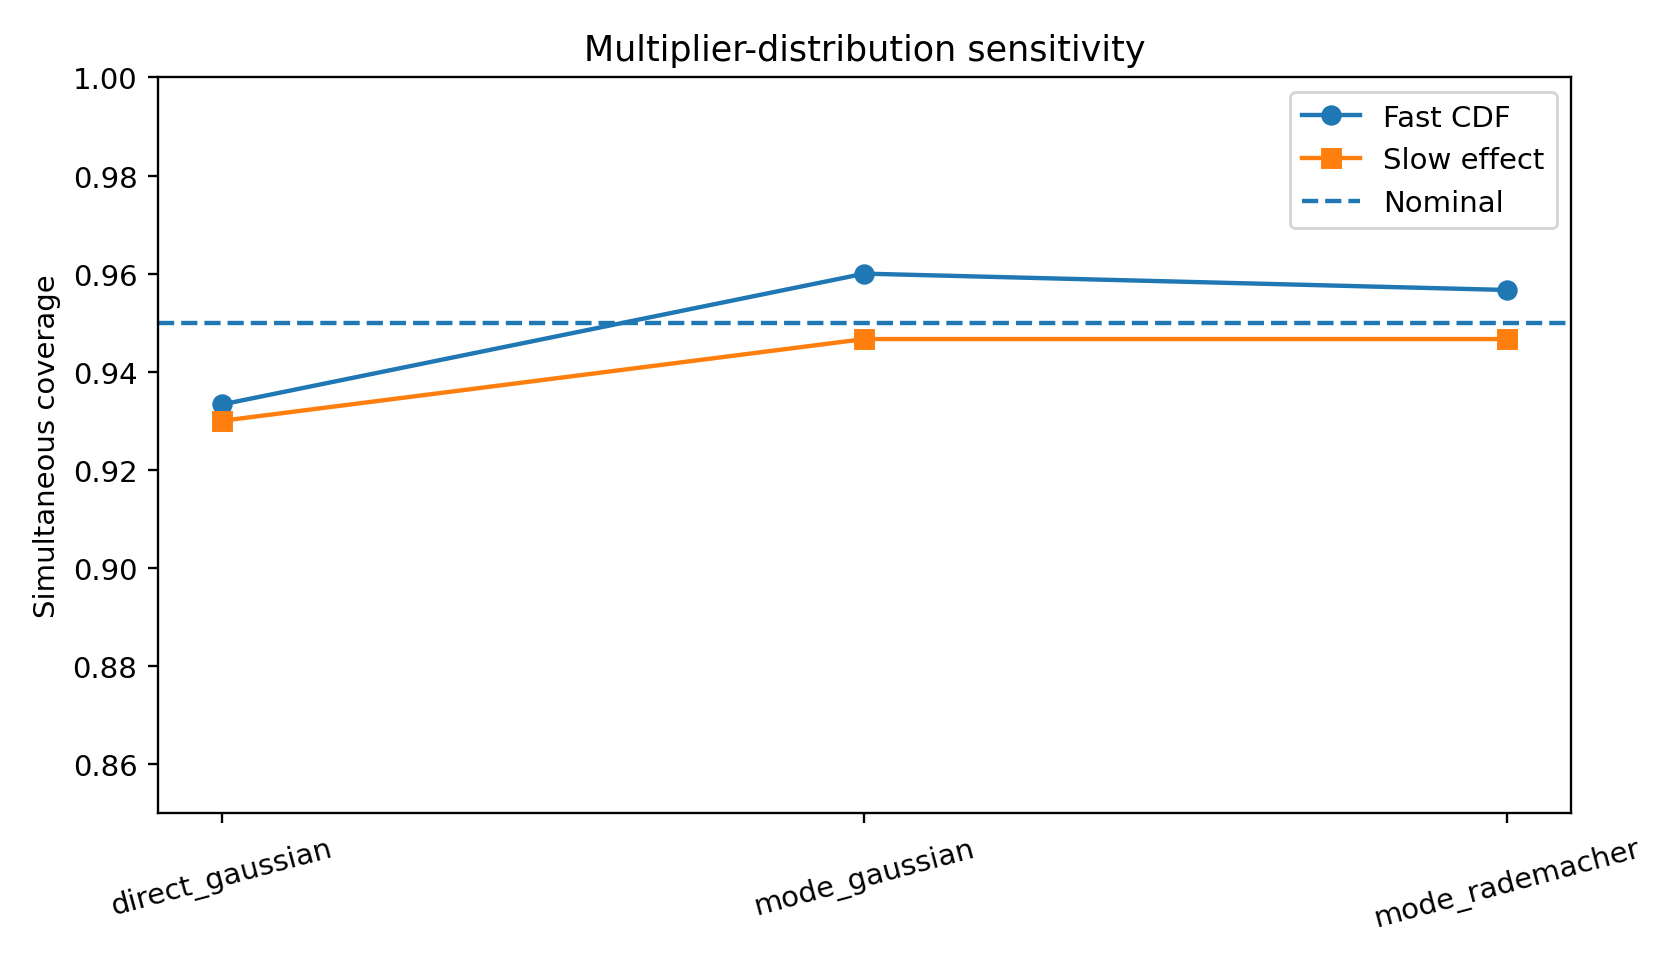
\includegraphics[width=.74\textwidth]{../results/figures/bootstrap_multiplier_sensitivity.png}
\caption{Simultaneous coverage by multiplier implementation.}
\end{figure}

\section{Galerkin, temporal, and total error}
\resizebox{\textwidth}{!}{%
\begin{tabular}{llllll}
\toprule
alpha\_q & metric & predicted\_slope & empirical\_slope & ci\_low & ci\_high \\
\midrule
0 & mean\_error & -2.6 & -2.58 & -2.595 & -2.565 \\
0 & variance\_error & -4.6 & -4.564 & -4.595 & -4.533 \\
0 & strong\_rms & -2.3 & -2.307 & -2.311 & -2.302 \\
0 & cdf\_sup & -2.6 & -2.58 & -2.595 & -2.565 \\
0.75 & mean\_error & -2.6 & -2.58 & -2.595 & -2.565 \\
0.75 & variance\_error & -6.1 & -6.082 & -6.259 & -5.905 \\
0.75 & strong\_rms & -2.6 & -2.587 & -2.598 & -2.575 \\
0.75 & cdf\_sup & -2.6 & -2.58 & -2.595 & -2.565 \\
1.5 & mean\_error & -2.6 & -2.58 & -2.595 & -2.565 \\
1.5 & variance\_error & -7.6 & -8.282 & -15.38 & -1.185 \\
1.5 & strong\_rms & -2.6 & -2.58 & -2.595 & -2.565 \\
1.5 & cdf\_sup & -2.6 & -2.58 & -2.595 & -2.565 \\
\bottomrule
\end{tabular}
}%


\begin{figure}[ht]
\centering
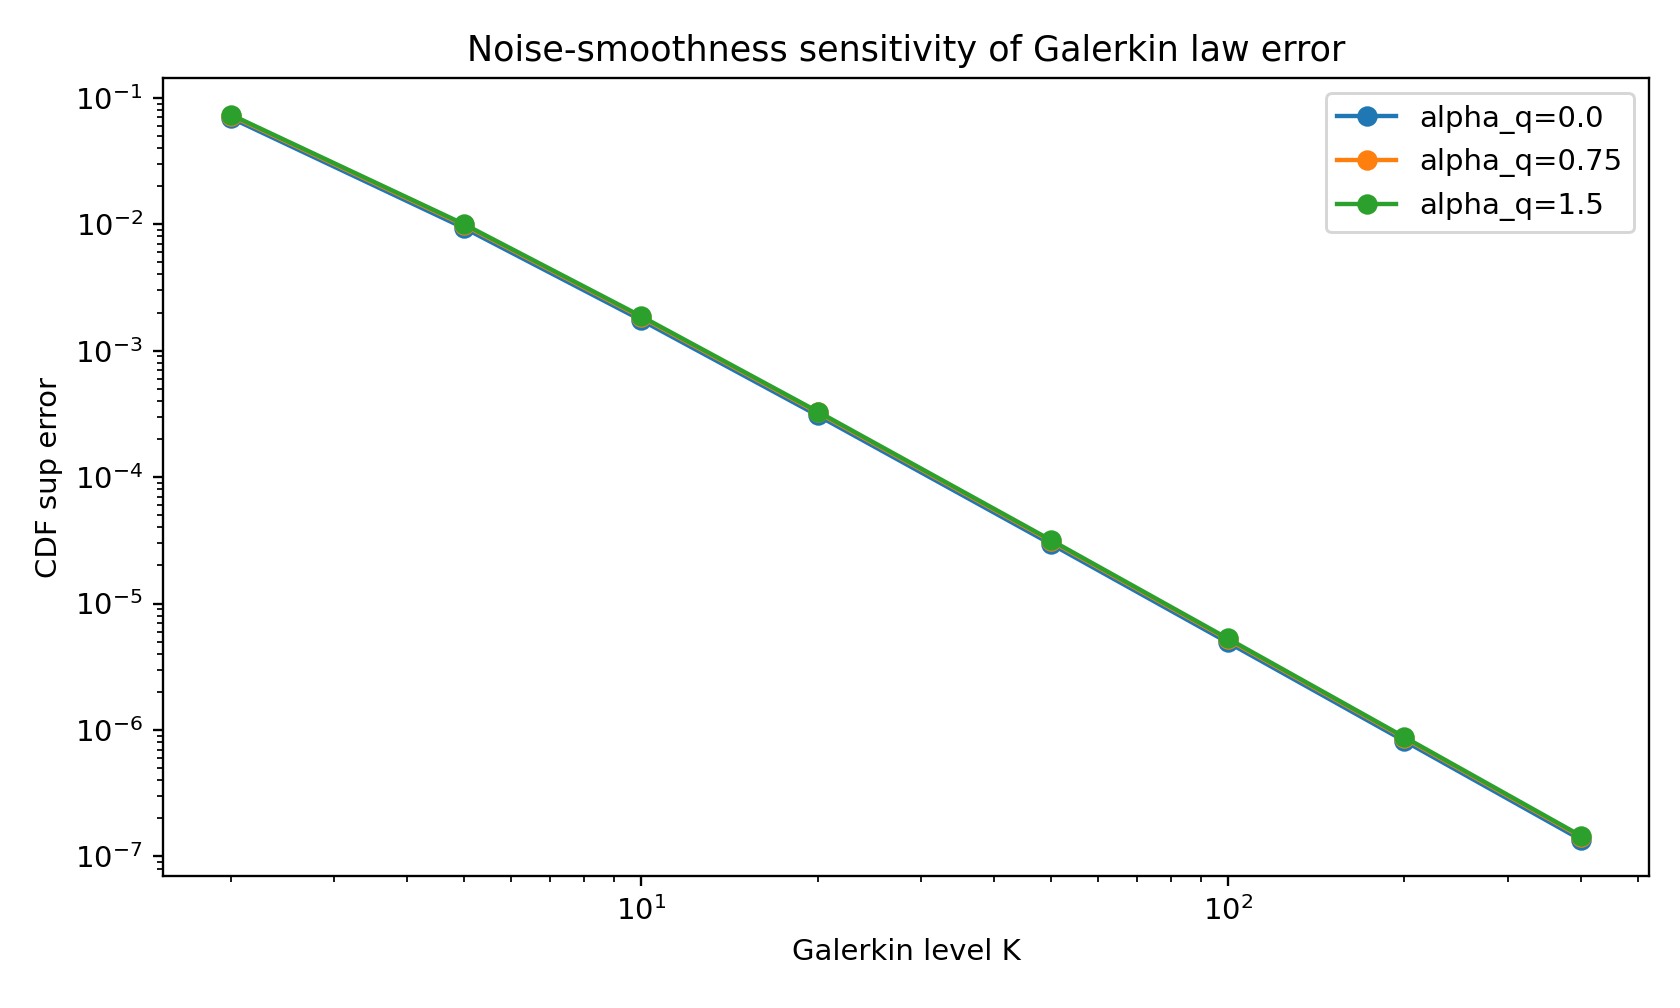
\includegraphics[width=.75\textwidth]{../results/figures/galerkin_alpha_rates.png}
\caption{Noise-smoothness sensitivity of the Galerkin CDF-law error.}
\end{figure}

\begin{figure}[ht]
\centering
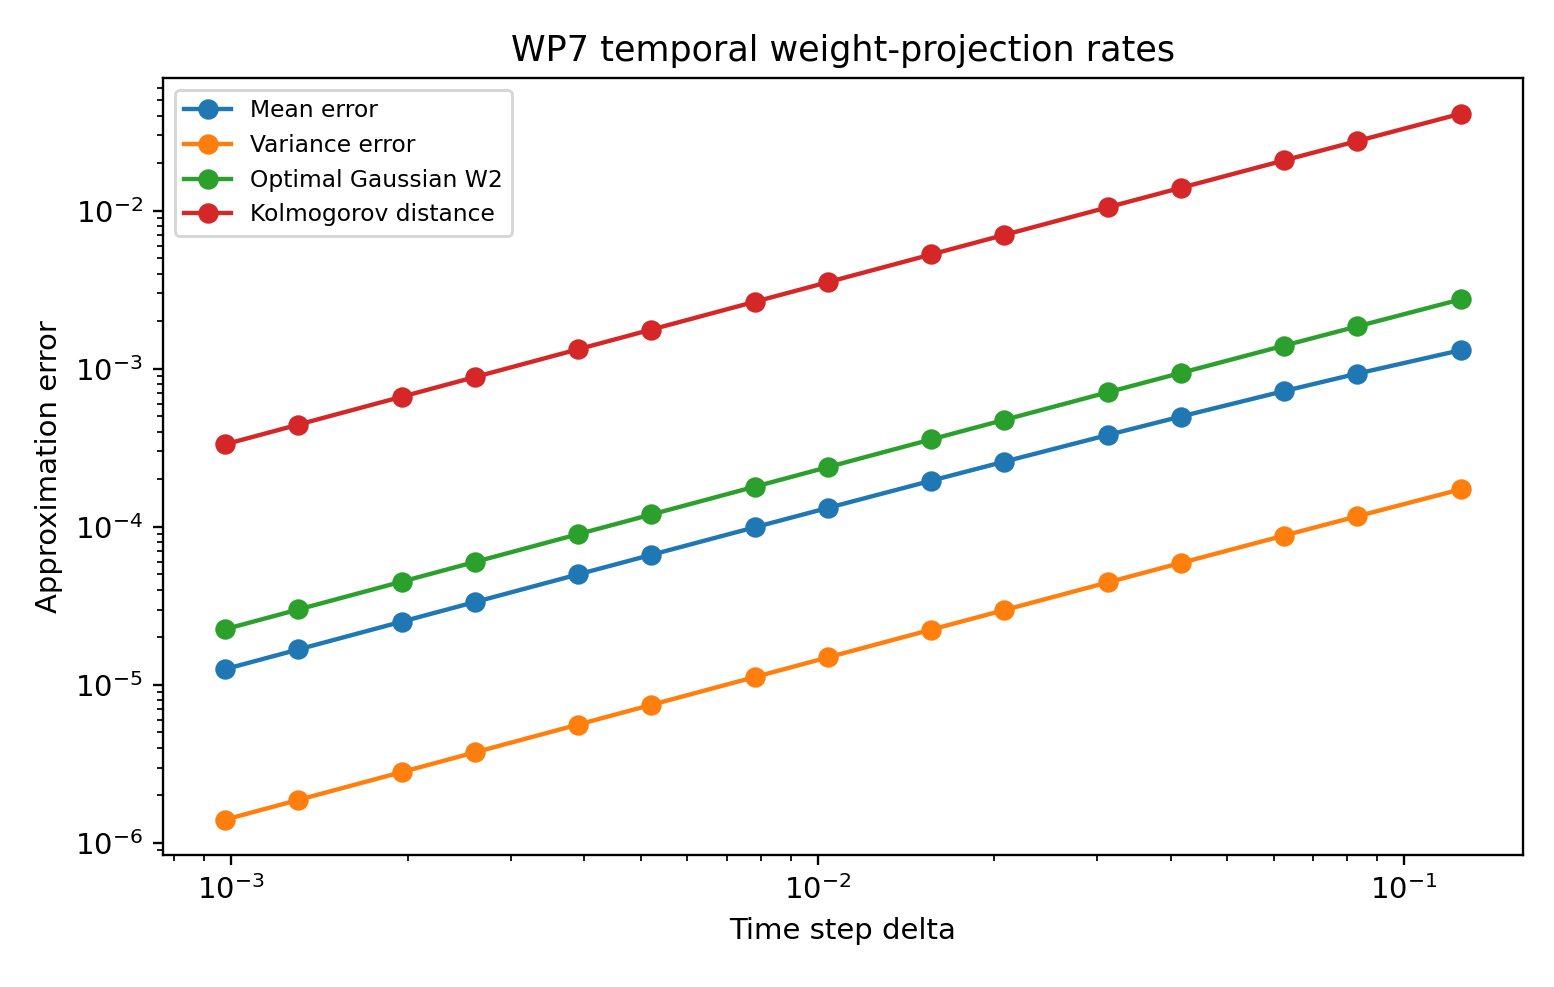
\includegraphics[width=.75\textwidth]{../results/figures/temporal_rates.png}
\caption{First-order temporal approximation rates.}
\end{figure}

\begin{figure}[ht]
\centering
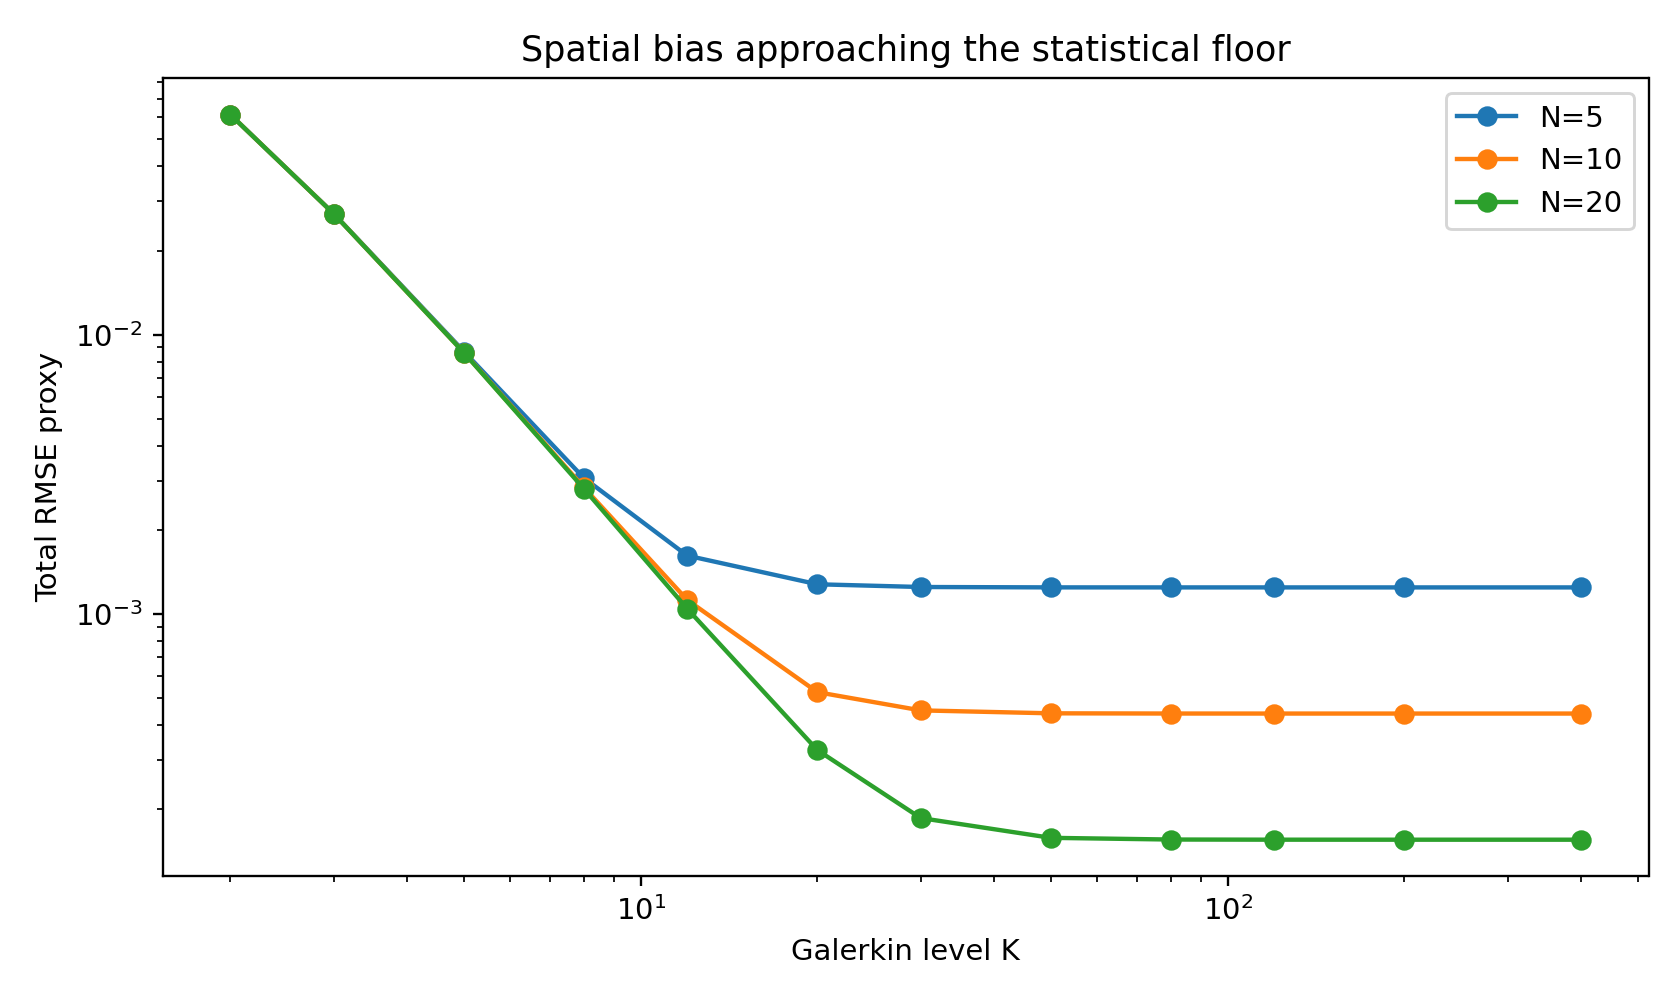
\includegraphics[width=.75\textwidth]{../results/figures/combined_error_balancing.png}
\caption{Truncation bias approaching the statistical error floor.}
\end{figure}

\begin{figure}[ht]
\centering
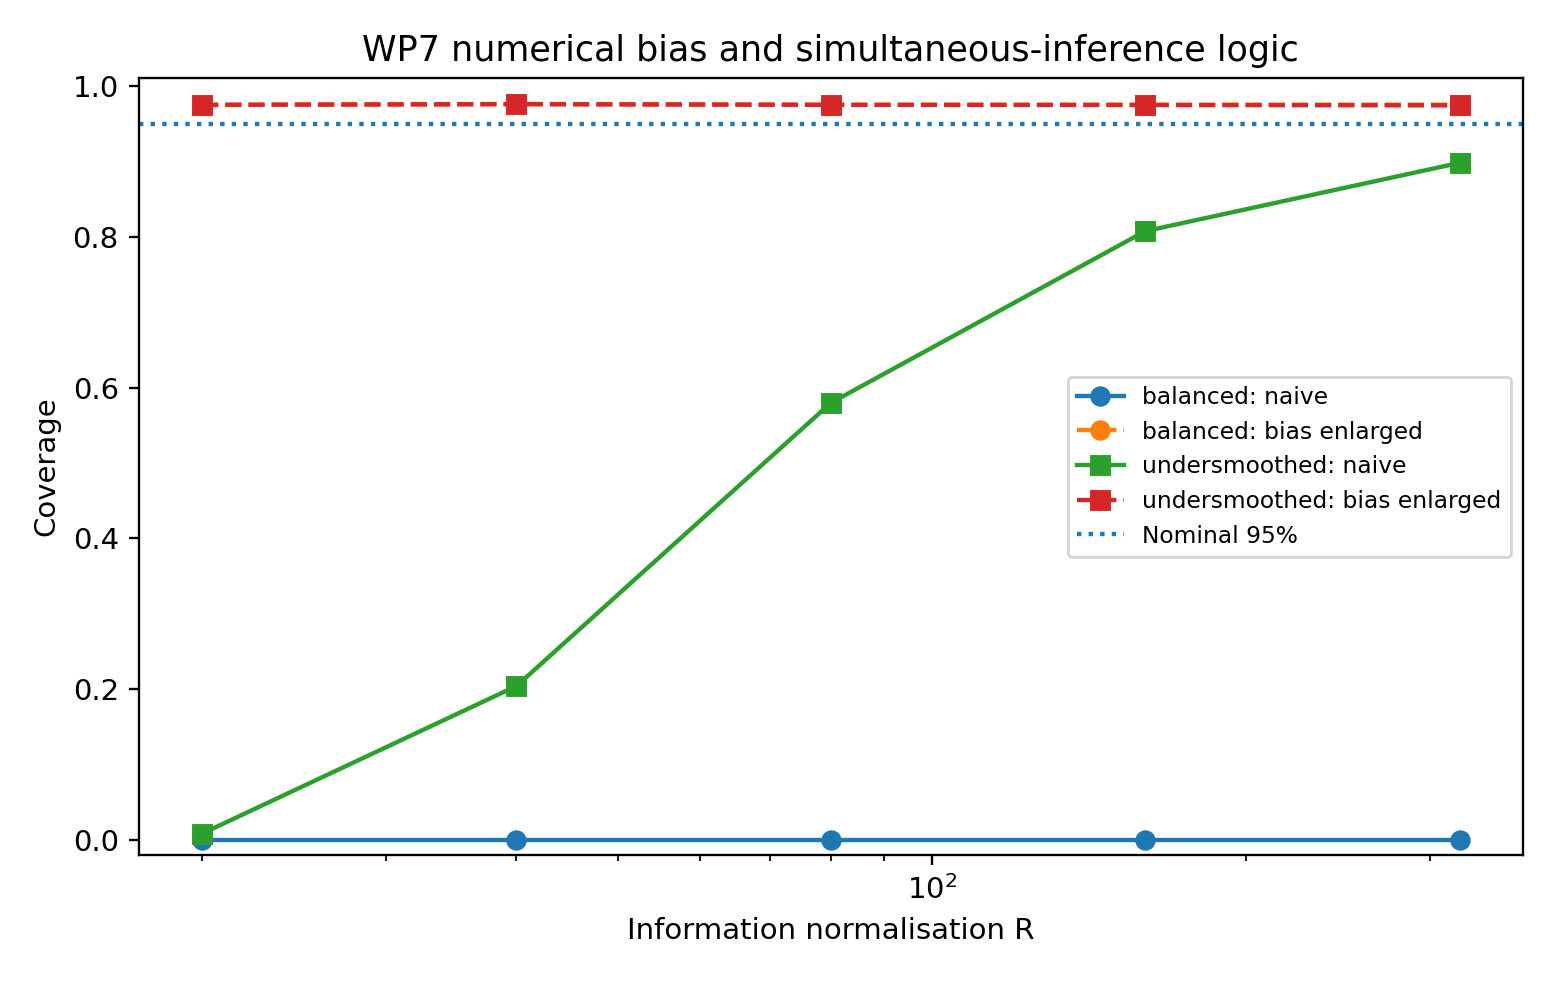
\includegraphics[width=.75\textwidth]{../results/figures/bias_coverage.png}
\caption{Naive and certified-bias-enlarged coverage.}
\end{figure}

\section{Operator sensitivity}
The central difference error falls from 4.270e-06 to 1.708e-09. The first-order CDF remainder is quadratic and the Wasserstein distance stays below the common-noise bound.

\begin{figure}[ht]
\centering
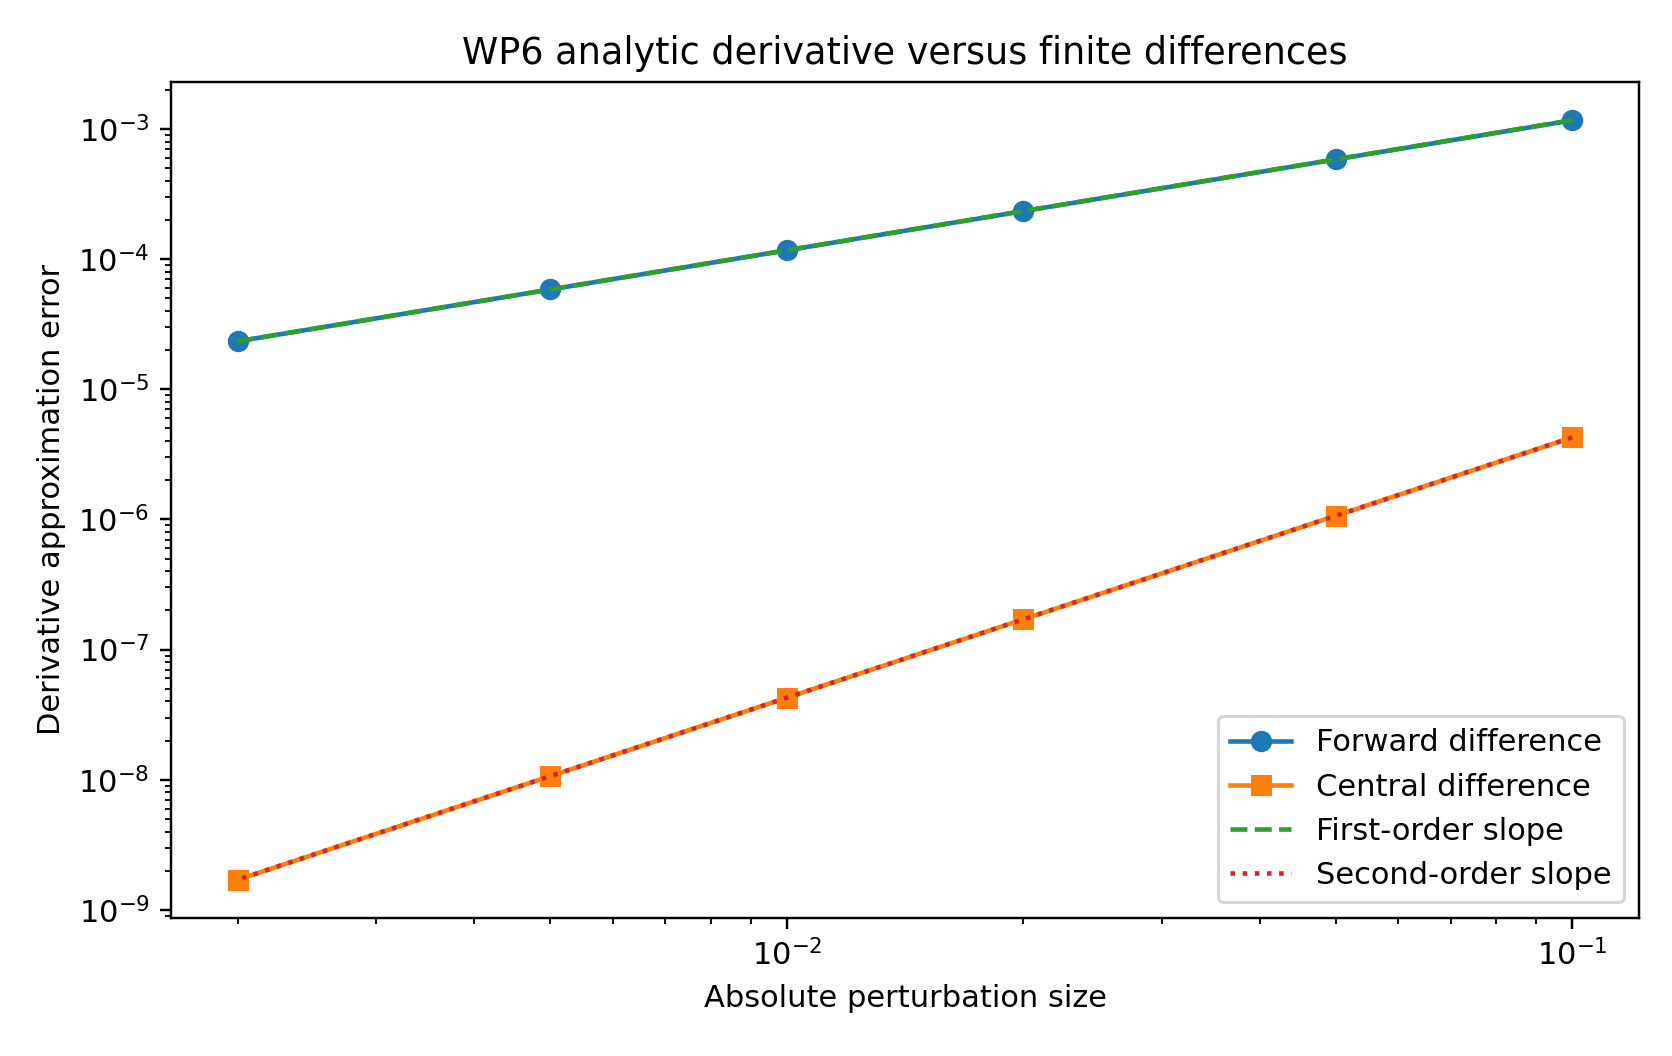
\includegraphics[width=.75\textwidth]{../results/figures/operator_finite_difference.png}
\caption{Finite-difference validation of the operator-law derivative.}
\end{figure}

\section{Non-identification}
The finite-grid open-loop example has factual covariance discrepancy 8.185e-16 and post-intervention discrepancy 0.7003.

\begin{figure}[ht]
\centering
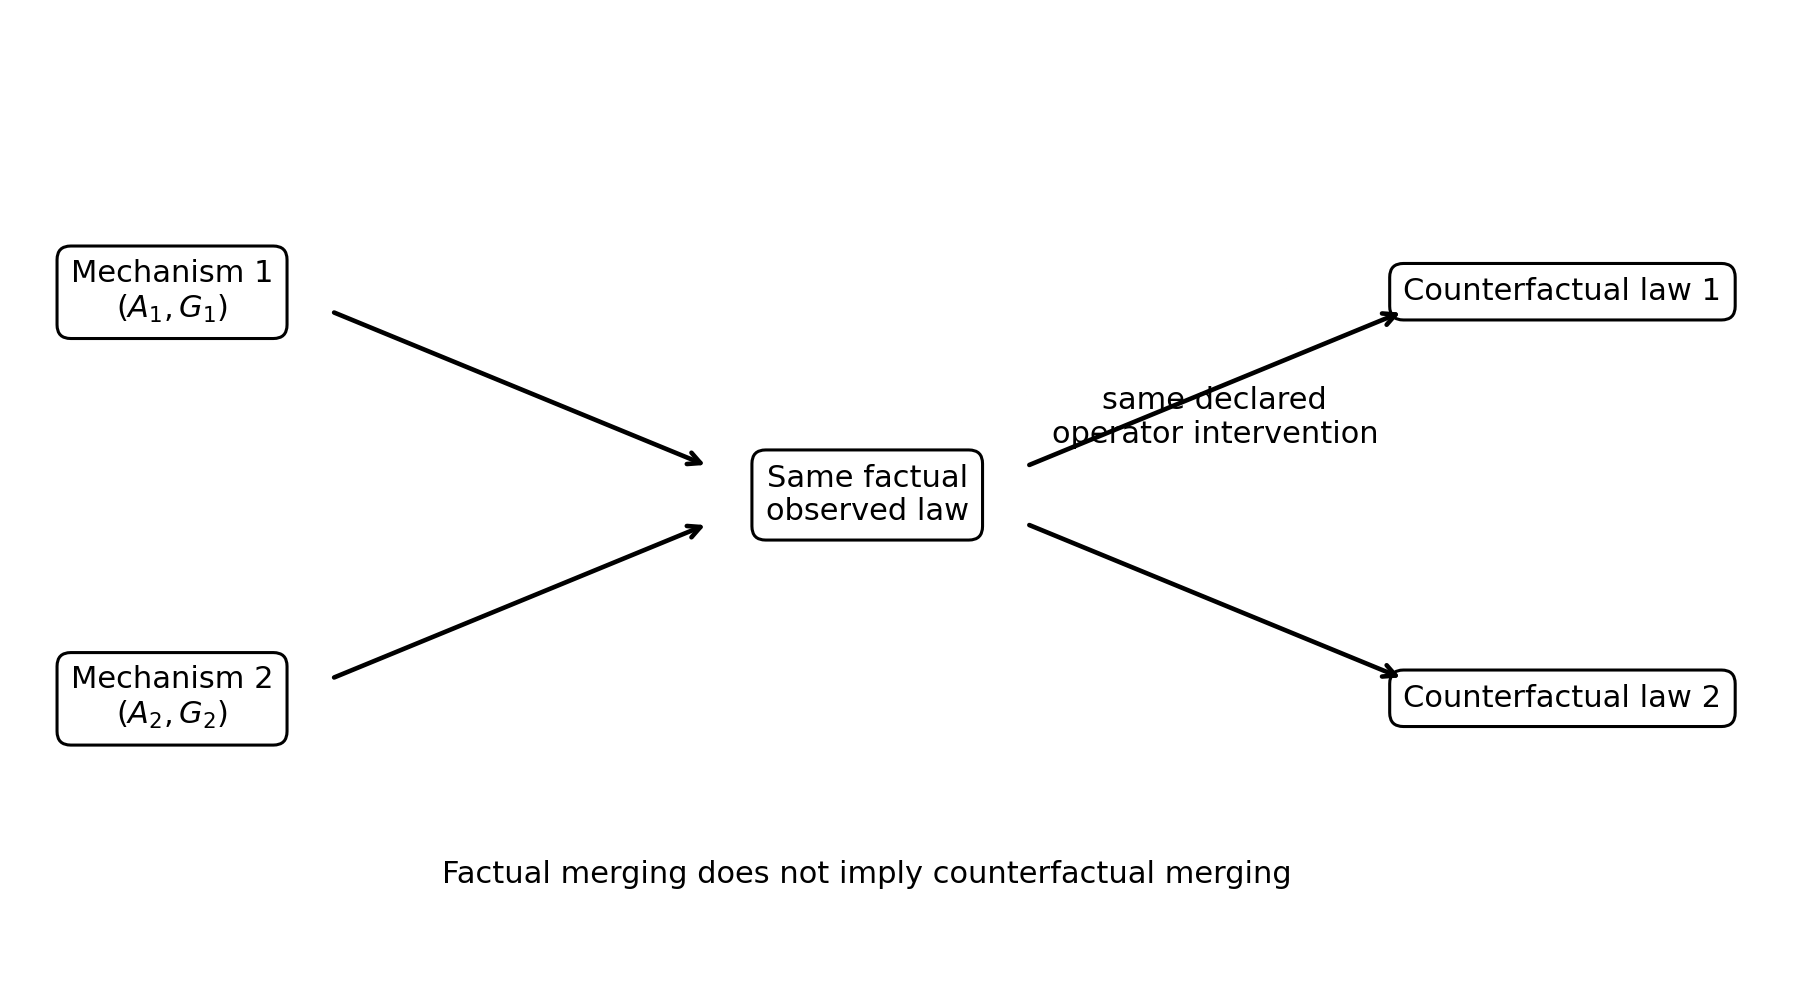
\includegraphics[width=.75\textwidth]{../results/figures/nonidentification_diagram.png}
\caption{Factual merging followed by counterfactual separation.}
\end{figure}

\begin{figure}[ht]
\centering
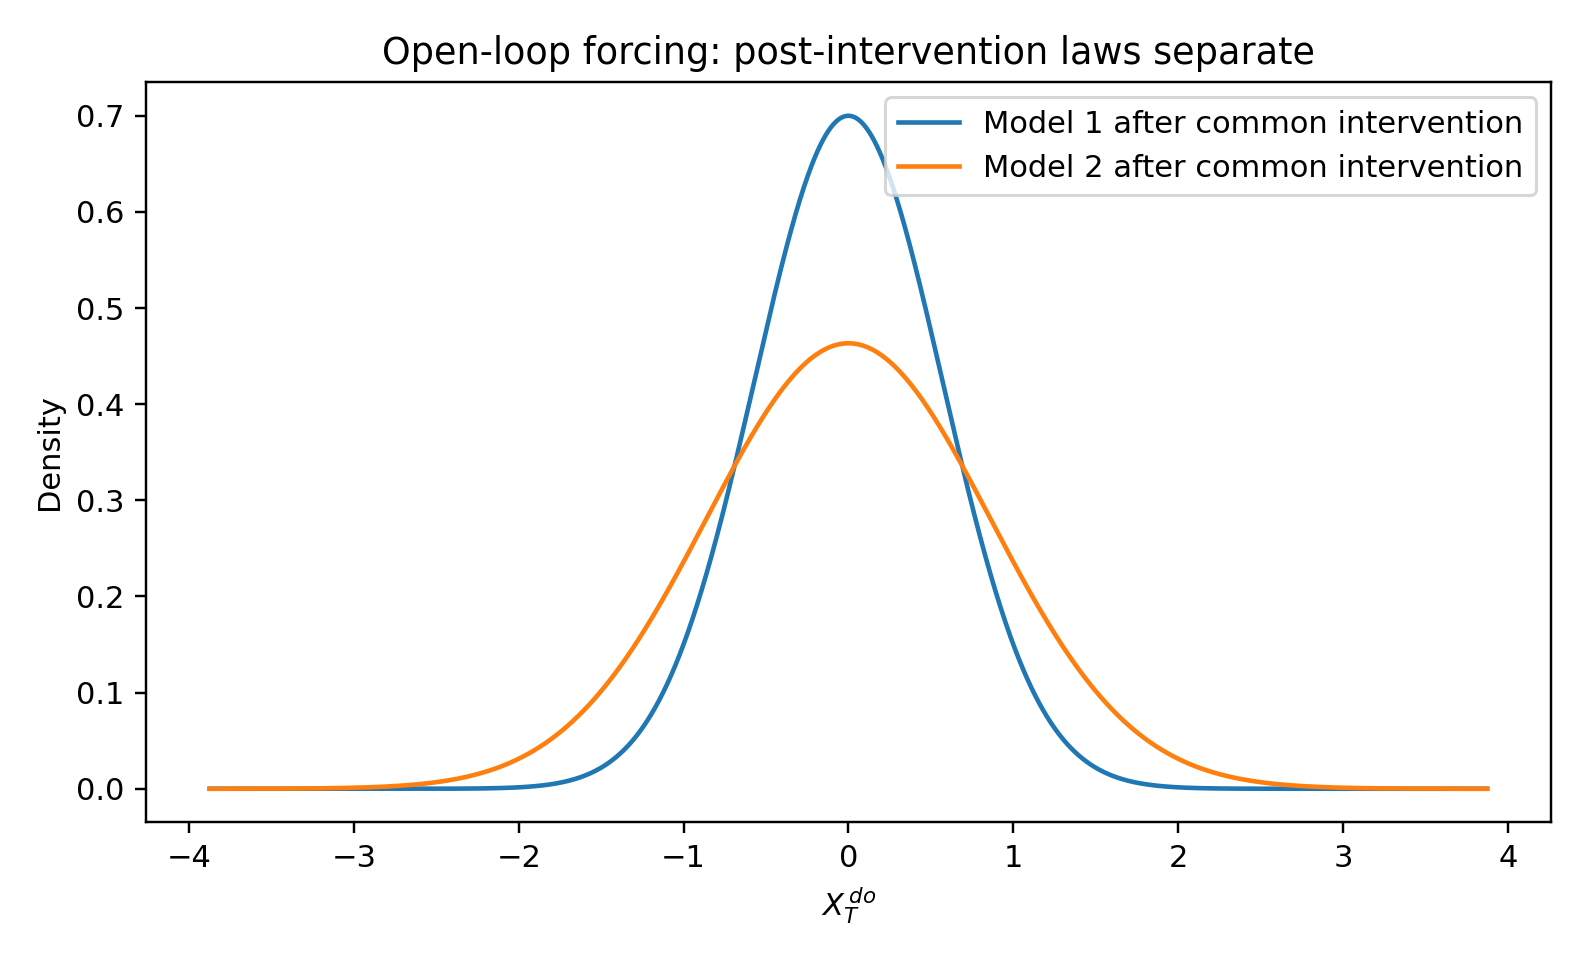
\includegraphics[width=.75\textwidth]{../results/figures/exogenous_counterfactual_split.png}
\caption{Open-loop forcing: separated post-intervention laws after exact factual equivalence.}
\end{figure}

\section{Completion gate and reproducibility}
\resizebox{\textwidth}{!}{%
\begin{tabular}{lrl}
\toprule
criterion & passed & diagnostic \\
\midrule
theorem\_aligned\_designs & True & 0.1234 \\
at\_least\_1000\_reps & True & 1000 \\
standardised\_sd\_near\_one & True & 0.02187 \\
simultaneous\_coverage\_reported & True & 7 \\
rate\_slopes\_checked & True & 0.6822 \\
operator\_remainder\_checked & True & 4.675e-08 \\
failure\_cases\_demonstrated & True & 0.7003 \\
planned\_grid\_audited & True & 1 \\
one\_command\_runner & True & 1 \\
\bottomrule
\end{tabular}
}%

The suite is executed with \texttt{make wp9}. It stores the full configuration, raw estimator replicates, summary tables, figures, environment metadata, the source commit, and SHA-256 checksums.

\end{document}
